\documentclass[11pt]{article}
\usepackage[margin=1in]{geometry}
\usepackage{graphicx}
\usepackage{amsmath}
\usepackage{booktabs}

\renewcommand{\topfraction}{0.95}
\renewcommand{\bottomfraction}{0.95}
\renewcommand{\textfraction}{0.05}
\setlength{\textfloatsep}{12pt plus 2pt minus 2pt}
\setlength{\intextsep}{12pt plus 2pt minus 2pt}
\setlength{\floatsep}{12pt plus 2pt minus 2pt}






\title{Mean Residual Correction: A Finite Worked Example}
\author{Anonymous}
\date{}

\begin{document}
\raggedbottom
\maketitle

\begin{abstract}
An additive intercept correction provides a compact setting for distinguishing an optimum from exact fit, and observed agreement from identification of a target function. For five supplied synthetic observations, targets are $2x+3$ and baseline predictions are $2x$. The mean residual is $3$; adding it reduces recorded mean squared error from $9$ to $0$. We connect the squared-error decomposition to executable arithmetic, a dependency diagram, and self-checks whose solutions state the conditions for zero error and global equality.
\end{abstract}

\section{Introduction}

The intended reader knows elementary algebra with affine functions, finite averages, and squared errors, and is beginning to interpret fitted predictions. The note targets two inference errors: treating zero mean residual as zero error, and extending agreement on fitting inputs to all inputs. Readers should be able to state the additional premise that makes each conclusion valid.

The instructional sequence links a decomposition, a computation, and a dependency diagram. The self-checks in Section~\ref{sec:checks} express the learning objectives through explicit mathematical answers and solution criteria.

\section{Related Work}

The relevant viewpoints are least-squares intercept fitting, residual centering, and interpolation. Intercept fitting holds the baseline predictor fixed and optimizes an additive scalar; centering describes the residuals after that optimization; interpolation concerns agreement with observed target values. These viewpoints answer different questions within the same calculation.

The expository focus is their connection: the minimizing offset alone does not explain zero remaining error, and exact fit acquires a global interpretation after specifying a target function class. Figure~\ref{fig:residual-workflow} connects these questions to the targets used for fitting and evaluation.

\section{Method}

\subsection{Finite Construction and Scalar Correction}
\label{sec:construction}

For the ordered inputs $\mathbf{x}=(-2,-1,0,1,2)$, define
\[
y_i=2x_i+3,\qquad
\hat{y}^{(0)}_i=2x_i,\qquad
r_i=y_i-\hat{y}^{(0)}_i=3.
\]
On $\mathcal{D}=\{(x_i,y_i)\}_{i=1}^{5}$, the correction and corrected predictor are
\[
\bar r=\frac{1}{5}\sum_{i=1}^{5}r_i=3,
\qquad
\hat{y}_i(b)=2x_i+b.
\]
Within the fixed-slope, constant-offset target class, any one observed pair determines the offset $3$. The other four repeat that intercept information while making averaging and evaluation explicit.

\subsection{Residual Decomposition and Error Definitions}

For any finite residual list $r_1,\ldots,r_n$, with $n\geq1$, let
$\bar r=n^{-1}\sum_i r_i$. Expanding
$r_i-b=(r_i-\bar r)+(\bar r-b)$ gives
\[
\begin{aligned}
\operatorname{MSE}(b)
&=\frac{1}{n}\sum_{i=1}^{n}(r_i-b)^2\\
&=\frac{1}{n}\sum_{i=1}^{n}(r_i-\bar r)^2
  +(b-\bar r)^2.
\end{aligned}
\]
The cross term vanishes because $\sum_i(r_i-\bar r)=0$.
Thus $b=\bar r$ uniquely minimizes MSE. The minimum is residual variance with divisor $n$; it is zero exactly when every original residual equals $\bar r$. Subtracting the mean always centers residuals; eliminating them additionally requires this equality condition.

For the supplied constant residuals,
\[
\begin{aligned}
\operatorname{MAE}_{\mathcal{D}}(b)
&=\frac{1}{5}\sum_{i=1}^{5}|r_i-b|=|3-b|,\\
\operatorname{MSE}_{\mathcal{D}}(b)
&=\frac{1}{5}\sum_{i=1}^{5}(r_i-b)^2=(3-b)^2.
\end{aligned}
\]

\begin{figure}[!htbp]
\centering
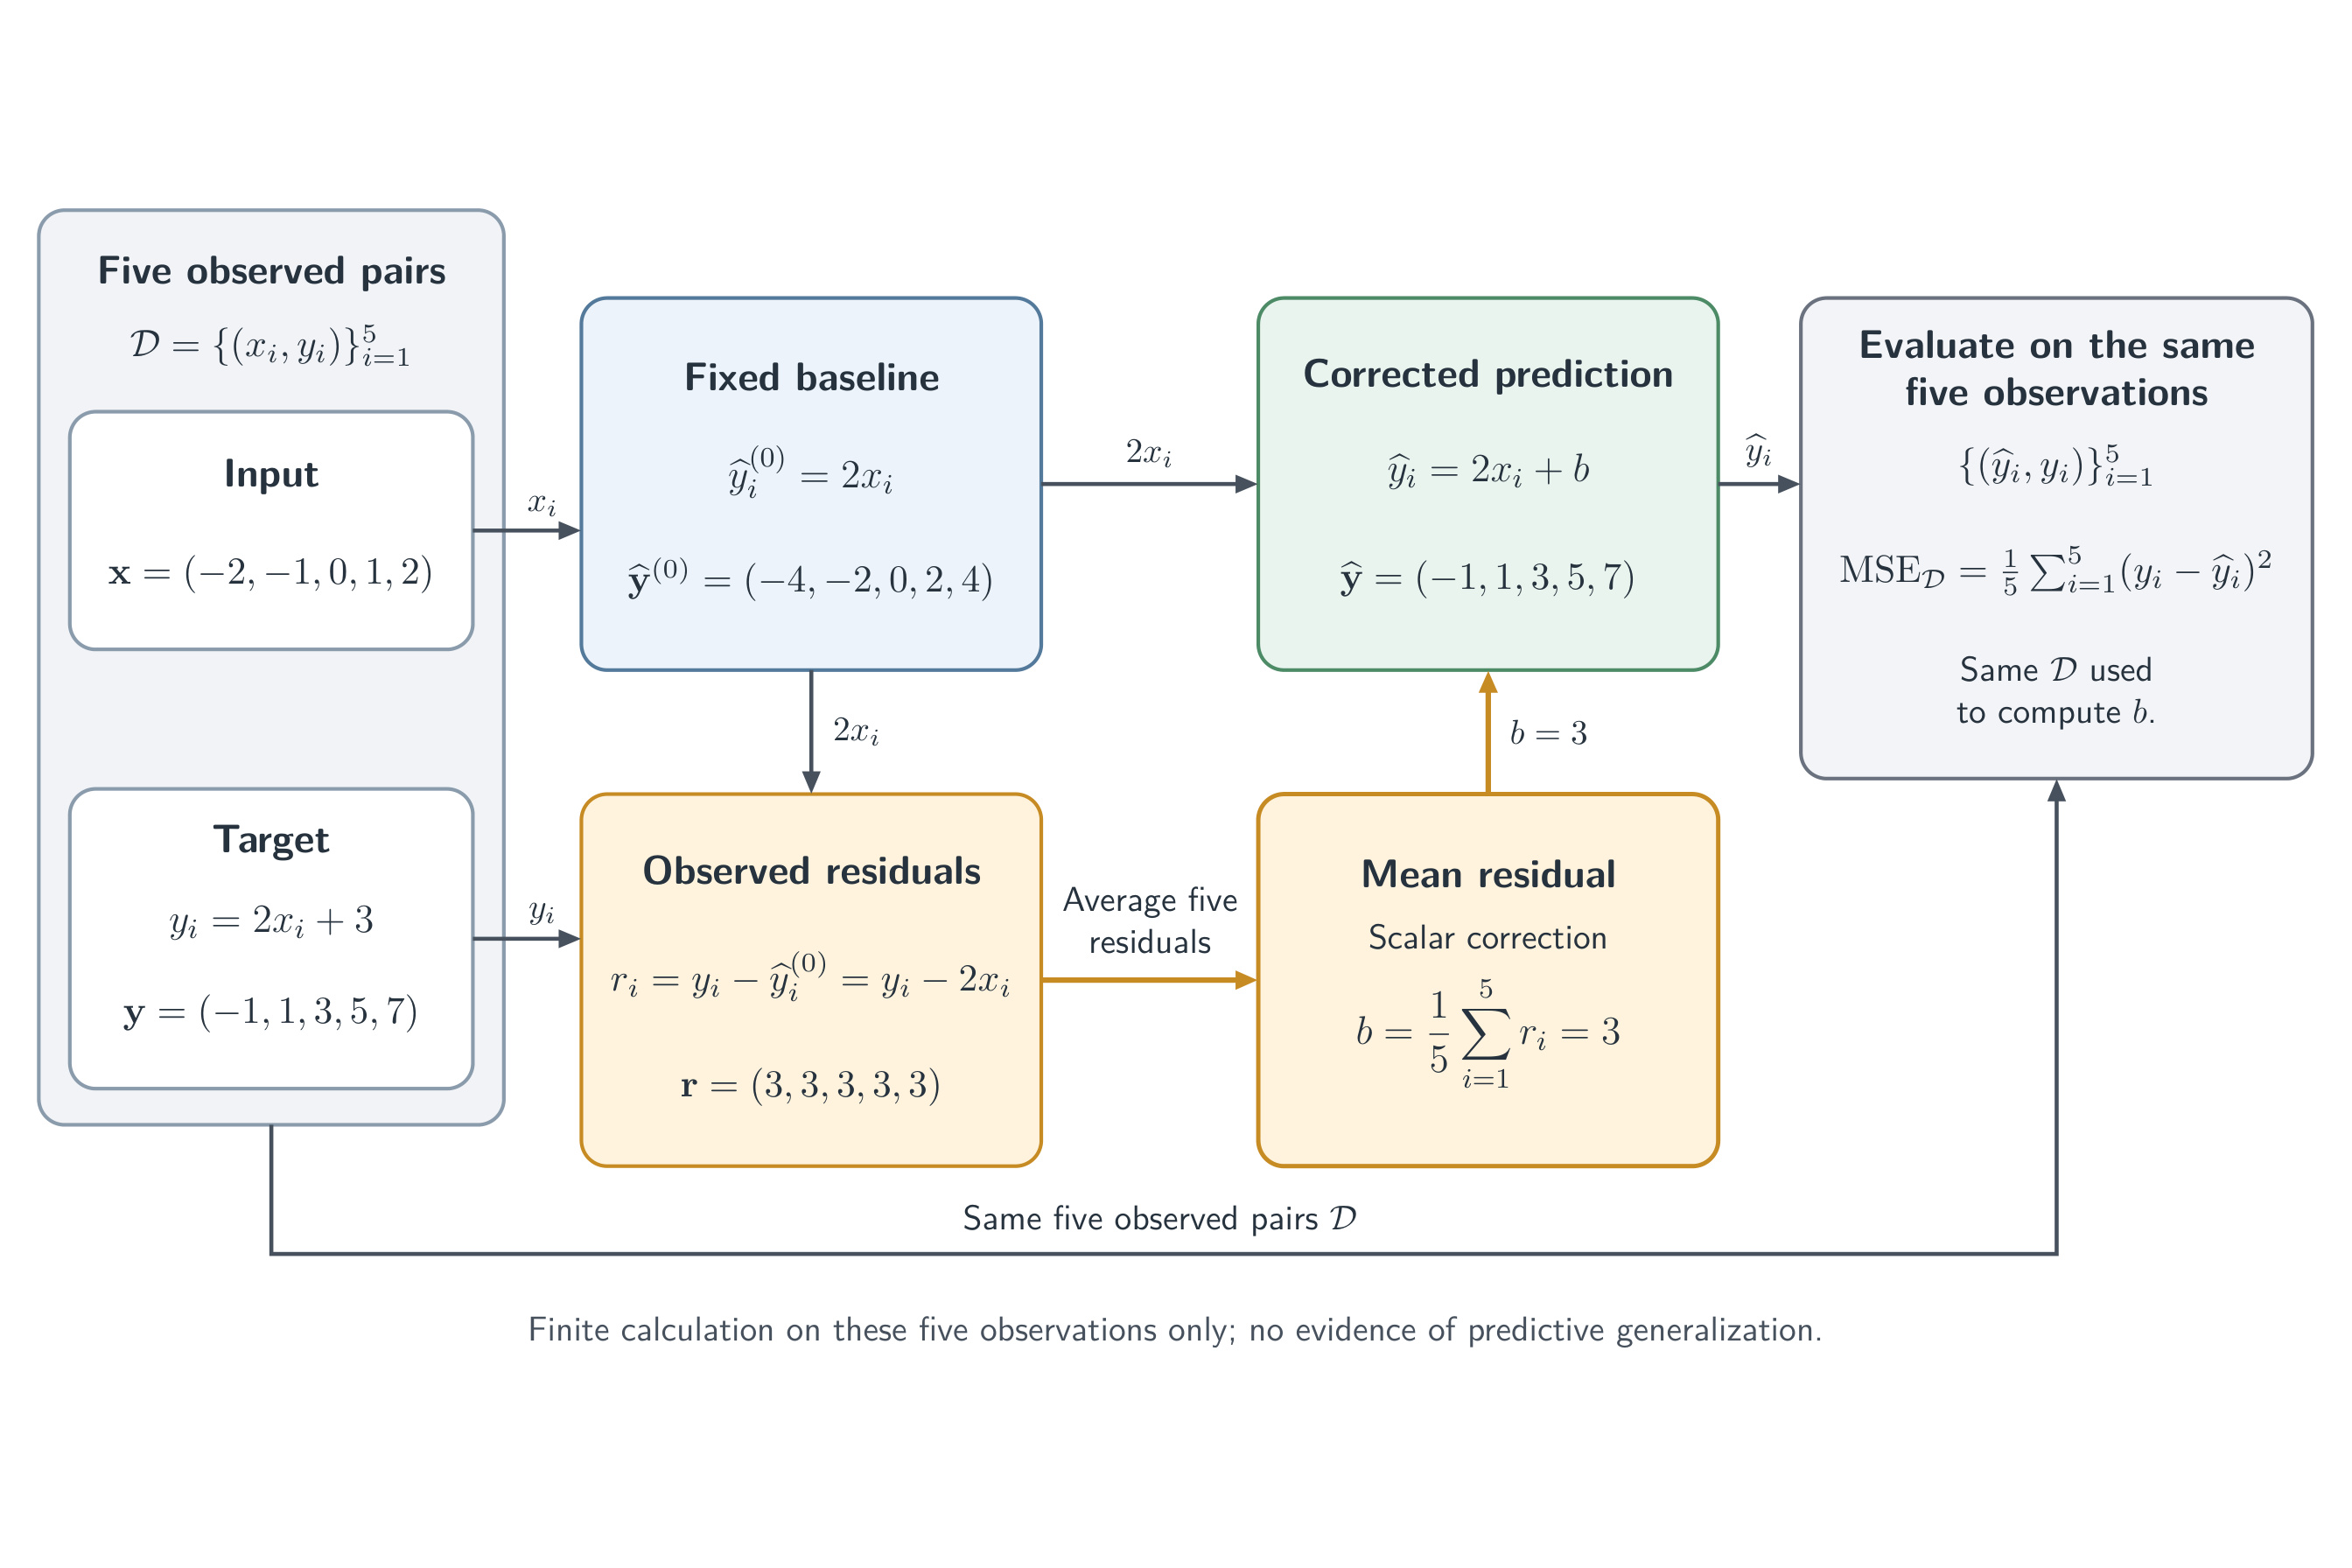
\includegraphics[width=\linewidth]{figures/fig_residual_workflow.jpg}
\caption{Targets and baseline predictions determine residuals; their mean determines $b=3$. The evaluation reuses the same five targets.}
\label{fig:residual-workflow}
\end{figure}

\section{Experiments: A Worked Example}

\subsection{Recorded Arithmetic}

The target, baseline, and corrected vectors are
$(-1,1,3,5,7)$, $(-4,-2,0,2,4)$, and $(-1,1,3,5,7)$, respectively. This Base R listing reproduces the correction and Table~\ref{tab:recorded-errors}:
\begin{quote}
\begin{minipage}{\linewidth}
\small
\begin{verbatim}
x <- c(-2, -1, 0, 1, 2)
y <- 2*x + 3
r <- y - 2*x
b <- mean(r)
offset <- c(0, 1.5, b)
errors <- vapply(offset, function(a) {
  e <- y - (2*x + a)
  c(MAE = mean(abs(e)), MSE = mean(e^2))
}, numeric(2))
cbind(b = offset, t(errors))
\end{verbatim}
\end{minipage}
\end{quote}

\subsection{Recorded Errors and Interpretation}

Table~\ref{tab:recorded-errors} and Figure~\ref{fig:intercept-error} show the three recorded offsets: the baseline, a prescribed partial correction, and the mean correction. At $b=1.5$, each residual becomes $1.5$, MAE halves, and MSE falls from $9$ to $2.25$. At $b=3$, both errors equal zero. These are errors on the observations used to determine the correction, as Figure~\ref{fig:residual-workflow} makes explicit.

\begin{table}[!htbp]
\centering
\caption{Recorded errors on the five observations used to determine the mean correction.}
\label{tab:recorded-errors}
\begin{tabular}{rrr}
\toprule
Added $b$ & Mean absolute error & Mean squared error \\
\midrule
0   & 3   & 9    \\
1.5 & 1.5 & 2.25 \\
3   & 0   & 0    \\
\bottomrule
\end{tabular}
\end{table}

\begin{figure}[!htbp]
\centering
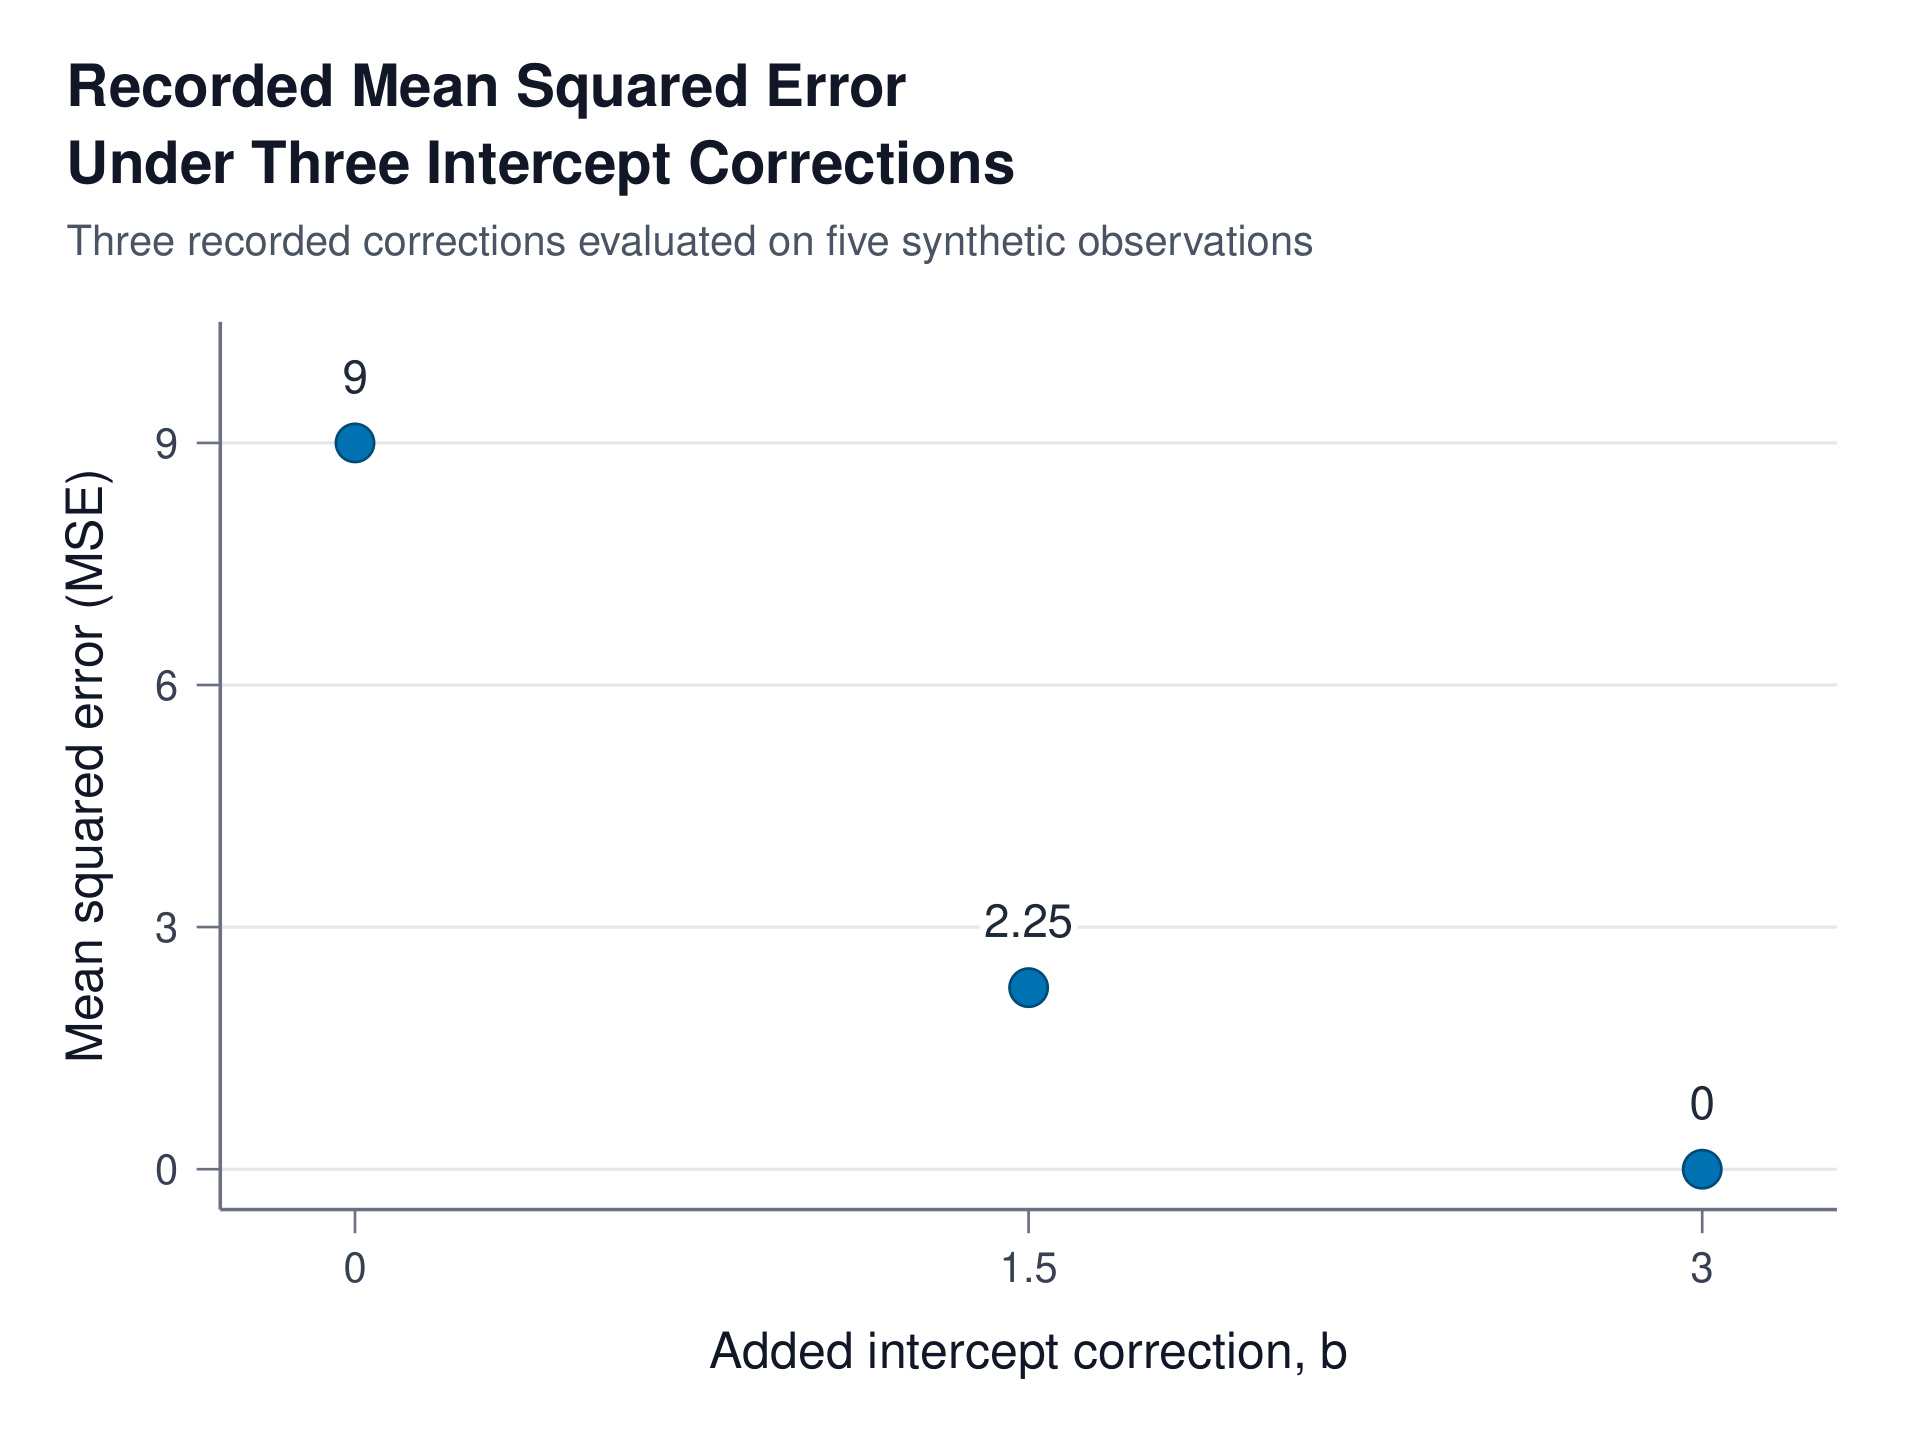
\includegraphics[width=0.92\linewidth]{figures/fig_intercept_error.jpg}
\caption{The three recorded MSE values: $9$, $2.25$, and $0$ at offsets $0$, $1.5$, and $3$. Each point uses the same five supplied targets.}
\label{fig:intercept-error}
\end{figure}

\subsection{Guided Self-Checks}
\label{sec:checks}

\paragraph{Centering.}
For the algebraic residual pair $(m-d,m+d)$, with $d\ne0$, derive the mean correction and remaining error:
\[
\bar r=m,\qquad
(r_1-\bar r,r_2-\bar r)=(-d,d),\qquad
\operatorname{MSE}(b)=d^2+(b-m)^2.
\]
The corrected residuals sum to zero, yet the minimum MSE is $d^2>0$. A complete explanation identifies cancellation in the signed sum and positivity in the sum of squares. This symbolic check isolates the equality condition in the decomposition.

\paragraph{Target identification.}
Construct target rules agreeing on all supplied inputs but differing elsewhere. For unrestricted functions, a symbolic answer is
\[
y_c(x)=2x+3+c\,x(x^2-1)(x^2-4),
\qquad c\ne0.
\]
The added product vanishes at every supplied input and is nonzero at every other real input. Each rule therefore gives the same five targets, correction, and recorded errors.

Now restrict the target to the affine class $y(x)=ax+k$. The supplied pairs $(0,3)$ and $(1,5)$ imply $k=3$ and $a+k=5$, hence $a=2$. They uniquely identify $2x+3$ within this class. Restricting the slope to $2$ beforehand gives the one-observation identification in Section~\ref{sec:construction}. The affine assumption excludes the nonzero polynomial term. Thus $\hat y(x)=2x+3=y(x)$ for every real $x$ follows from the supplied values together with that assumption.

\paragraph{Solution criteria.}
A complete solution distinguishes zero sum from zero sum of squares, reproduces the recorded table, traces target reuse in Figure~\ref{fig:residual-workflow}, and states the function-class premise permitting global equality.

\section{Conclusion}

The mean residual uniquely minimizes squared error; identical residuals make this minimum zero. The worked example connects that distinction to target identification: observed agreement determines an affine rule under the affine assumption, while the polynomial construction preserves alternative unrestricted rules.

% PAPER_ORCHESTRA_PROVENANCE_BEGIN
\clearpage
\section*{Figure source provenance}
The files below are the exact sources that produced the embedded figure previews. Paths are relative to this manuscript's source directory. The accompanying \texttt{figure\char95{}provenance.json} records all artifact checksums.\par
\medskip\noindent\textbf{Figure~\ref{fig:intercept-error} (\texttt{fig\char95{}intercept\char95{}error.jpg}).}\par
\noindent R/ggplot2 source: \texttt{figure\char95{}code/\allowbreak{}fig\char95{}intercept\char95{}error/\allowbreak{}source.R}.\par
\noindent Source SHA256: \texttt{279a7d4e\allowbreak{}7d20eb0a\allowbreak{}6abffb82\allowbreak{}7f647ea3\allowbreak{}487b0c35\allowbreak{}e69e6197\allowbreak{}5a2e4105\allowbreak{}a07dbaf4}.\par
\noindent Rendering metadata: \texttt{figure\char95{}code/\allowbreak{}fig\char95{}intercept\char95{}error/\allowbreak{}render.json}.\par
\noindent Exact export wrapper: \texttt{figure\char95{}code/\allowbreak{}fig\char95{}intercept\char95{}error/\allowbreak{}worker.R}.\par
\noindent Wrapper SHA256: \texttt{6cb2b073\allowbreak{}27277f63\allowbreak{}fafbb553\allowbreak{}cd4f1f12\allowbreak{}c0f85bec\allowbreak{}37a49f3f\allowbreak{}a765da16\allowbreak{}a26b58ba}.\par
\noindent Rendering metadata: \texttt{figure\char95{}code/\allowbreak{}fig\char95{}intercept\char95{}error/\allowbreak{}sessionInfo.txt}.\par
\medskip\noindent\textbf{Figure~\ref{fig:residual-workflow} (\texttt{fig\char95{}residual\char95{}workflow.jpg}).}\par
\noindent LaTeX/TikZ source: \texttt{figure\char95{}code/\allowbreak{}fig\char95{}residual\char95{}workflow/\allowbreak{}source.tex}.\par
\noindent Source SHA256: \texttt{0e593c80\allowbreak{}5cefd9d6\allowbreak{}ce898527\allowbreak{}f7009807\allowbreak{}405f913c\allowbreak{}e88197b5\allowbreak{}1715f01f\allowbreak{}592cbfee}.\par
\noindent Rendering metadata: \texttt{figure\char95{}code/\allowbreak{}fig\char95{}residual\char95{}workflow/\allowbreak{}render.json}.\par
% PAPER_ORCHESTRA_PROVENANCE_END
\end{document}